\documentclass[12pt]{article}
\usepackage[backend=bibtex,style=numeric]{biblatex} 
\usepackage[breaklinks=true, bookmarks=false]{hyperref}

\usepackage{graphicx}

\addbibresource{references.bib} 

\title{Report for the CPS Final Project}
\author{
    Andrea Auletta \\ \texttt{andrea.auletta@studenti.unipd.it} \and
    Niccolò Zenaro \\ \texttt{niccolo.zenaro@studenti.unipd.it} \and 
    Reference paper: \\ \textbf{Attack taxonomies for the Modbus protocols} \cite{huitsing2008attack}
}
\begin{document}

\maketitle
\newpage
\tableofcontents
\newpage

\begin{abstract}
Modbus is a commonly used protocol in Supervisory Control And Data Acquisition (\textit{SCADA}) environments
for monitoring, control and data acquisition. Despite its wide popularity, Modbus is not secure because when it was developed and adopted ($1979$) security was not considered to be a concern in isolated Industrial Control Systems (\textit{ICS}), thus is not designed to be secure like modern IT networks.
Among the various attacks, 4 different taxonomies can be identified to facilitate formal risk analysis efforts for clarifying the nature and the scope of the security threats on Modbus systems and networks.
\end{abstract}

\section{Introduction and objectives}
\subsection{Modbus}
The Modicon Communication Bus (\textit{Modbus}) protocol operates in a master-slave or server-client based model. The master devices initiates the queries while the slave devices respond to all such queries.
Masters can either send a broadcast message to all the slaves or individually poll a specific device. 
All the experiments run in this work, like in the original paper \cite{huitsing2008attack} are focused on TCP/IP implementation, while the Modbus protocol 
can also be implemented on top of several communication networks, such as serial or UDP. 

Modbus TCP messages are wrapped in TCP/IP header and transmitted over an ethernet-based Modbus network 
between different devices. The \textit{Modbus Slaves} listen for incoming TCP connections on port 503, 
that was selected by us, and once a connection has been established the Protocol Data Unit (\textit{PDUs}) 
are exchanged and encapsulated in TCP messages. The protocol itself can be broken down into six sections: 
\begin{itemize}
    \item Transaction Identifier: a 2-byte field that is used to correlate request and responses; it is easily predictable due to poor randomization.
    \item Protocol identifier: a 2-byte field that for Modbus is always set to 0.
    \item Length: a 2-byte field that indicates the length of remaining bytes in the payload.
    \item Unit Identifier: 1 byte that is used to identify the specific slave at an IP address.
    \item Function Code: is a 1-byte field that indicates the action requested my master. For example, reading and writing coils, registers or holding registers.
    \item Data: this field has variable length, with values associated with the various function codes. 
\end{itemize}

\subsection{Attack identification}
In general, attacks on Modbus systems and networks can exploit protocol's specifications, i.e. they are common to all Modbus systems/networks that 
conform to the protocol specifications. The attack identification methodology used by the authors \cite{huitsing2008attack} involves an analysis of each protocol, that leads to four groups or threat categories: \textit{interception}, \textit{interruption}, \textit{modification}, \textit{fabrication}.
The main targets for the Modbus protocol are the master, the field device, the serial communication links and messages. Attacks were implemented based on the possibility of the system to have a Modbus sniffer and a packet injector, that also could block, modify or fabricate arbitrary Modbus messages or sequences of messages. 

Fifteen attacks that exploit TCP protocols have been recognized, and as said require access to the master device, network communication path or field device.
The most serious attacks are those that disable or bypass the master unit and seize control of field devices, this type of attacks affect the integrity and the availability of
messages or of the network; on the other hand attacks on confidentiality involve obtaining information on the network or on slave devices by simply reading messages.

\subsection{Objectives}
In this work we tried to replicate the various attacks defined by the authors, 
specifically we emulate one attack for each taxonomy identified in the paper. 
We built our own Modbus simulator with python libraries and then we produced python scripts for each attack.
More precisely, the \textit{interception}, \textit{interruption}, \textit{modification} and 
\textit{fabrication} identified in the original paper are described and implemented as follows:
\begin{itemize}
    \item Interception: \textit{Passive reconnaissance} involves passively reading Modbus messages or network traffic, intercepting the messages and reading field device data.
    \item Interruption: \textit{TCP FIN flood} is an interruption attack that aims to launch spoofed TCP packets with the FIN flag set after a legitimate message from Modbus server to Modbus client, in order to close the TCP connection or cause 
    significant delays.
    \item Modification: \textit{Response Delay} involves delaying a response message so that the master 
    receives out-of-date information from slaves, 
    is done by sniffing and modifying field device, sending the modified packet with a delay.
    \item Fabrication: \textit{Rogue Interloper} is a sort of man-in-the-middle attack where a MITM device can sniff and fabricate messages.
\end{itemize}

\section{System setup}
This work was entirely done with python scripts, crafting master and slaves with \href{https://pymodbus.readthedocs.io/en/latest/}{\texttt{PyModbus}} and working on TCP level with \href{https://scapy.readthedocs.io/en/latest/}{\texttt{Scapy}}.
Although these are two of the most famous python labraries for dealing with TCP Modbus packets, we found out that their documentation is often incomplete and not accurate, with most of the 
information difficult to retrieve. 

Wireshark was employed for sniffing the entire connection on the \texttt{Loopback interface} and on \texttt{port 503}, in order to obtain a feedback on what actually happened on our Modbus TCP network.

\section{Experiments, results and discussions}
In this section we describe the experiments done to emulate the attacks. 
All the scripts are available in the \texttt{code} folder of the \href{https://github.com/auli16/cpsProjectModBus}{Repository}.
We assume that the attacker knows IP address and the port where the devices are listening. 
First of all, in all the experiments we have a master and a slave except for the Fabrication where we need only the server.
The slave is a simple Modbus server that listens on port 503 and the master is a Modbus 
client that sends requests to the slave. So run the \texttt{slave.py} script on a terminal to start 
the server listening. In the file 
\texttt{master.py} there are three different function used to read, write coils and registers:
\begin{itemize}
    \item master\_read(): reads the data from all the registers of the slave;
    \item master\_connected(time\_wait): the master will be connected for 
    time\_wait seconds to the slave, it will read coils and will be disconnected time\_wait seconds;
    \item master\_write(): writes values in the holding registers of the slave.
\end{itemize}
One of these functions is called based on the attack type (change it in the main function of the file).
The master has to be run in a different terminal.
\subsection{Interception attack}
The goal of this attack is to intercept a sent message from the master to the slave. In the master, the function \texttt{master\_read()} is called. Before calling the master, run the \texttt{interception.py} script that will sniff the packet and print it. 
The attacker will listen to the network and, when it finds the packet with the right characteristics, 
it will print it.
\begin{figure}[h]
    \centering
    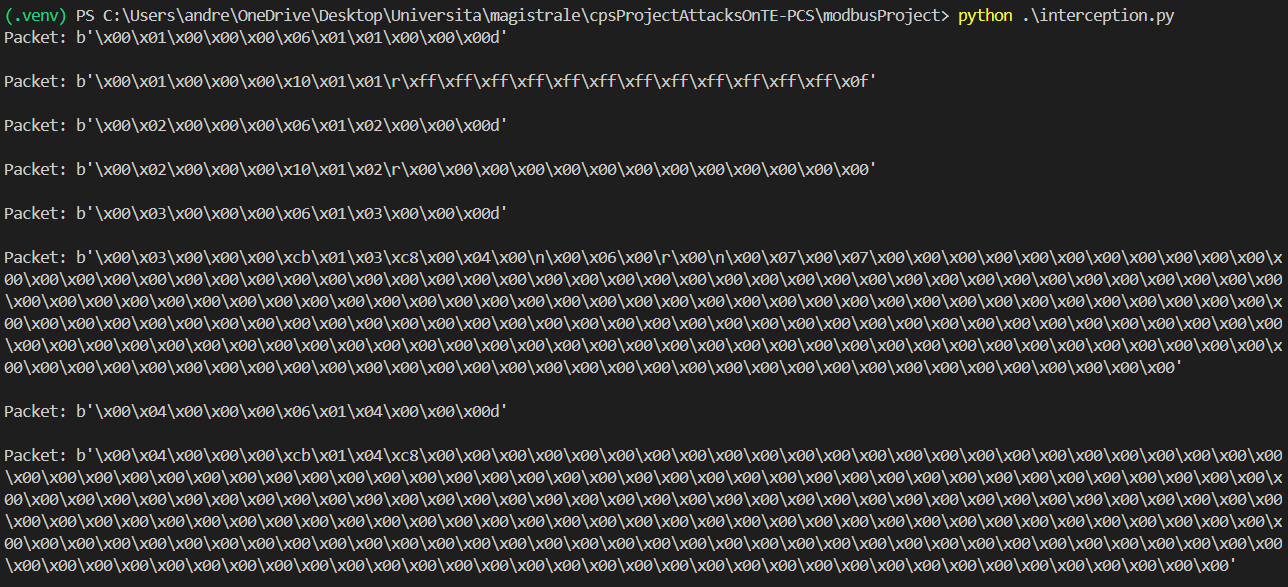
\includegraphics[width=1\textwidth]{images/InterceptionResults.png}
    \caption{Results of the interception attack}
    \label{fig:interceptionResult}
\end{figure}
In the image \ref{fig:interceptionResult} we can see that there are 4 operations requested by the master and 4 responses from the slave.
Here there is a conversion of the first packet present in the image:
\begin{enumerate}
    \item Transaction ID = x00x01 = 1;
    \item Protocol ID = x00x00 = 0;
    \item Length = x00x06 = 6;
    \item Unit ID = x01 = 1;
    \item Function Code = x01 = 1 (read coils);
    \item Data = x00x00x00;
\end{enumerate}
We found the function codes and their assignd functions in the following site \href{https://ozeki.hu/p_5873-modbus-function-codes.html}{codes}
\subsection{Fabrication attack}
The goal of this attack is to fabricate a fake message and send it to the server in order to change the value 
of a register, more precisely we substituted the value of the register 1 with 1337 of the holding registers.
For this attack, after starting the slave, run the \texttt{fabrication.py} script that will send the packet to the server.
In the following image \ref{fig:beforeFabrication} we can see the register of interest before the attack:
\begin{figure}[h]
    \centering
    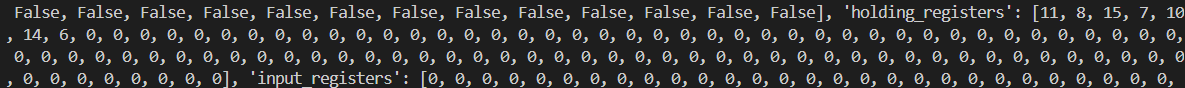
\includegraphics[width=1\textwidth]{images/BeforeFabrication.png}
    \caption{Register before the fabrication attack}
    \label{fig:beforeFabrication}
\end{figure}
A packet with the following characteristics is sent to the server:
\begin{enumerate}
    \item Transaction ID = x12x34 (chosen randomly);
    \item Protocol ID = x00x00 = 0;
    \item Length = x00x06 = 6;
    \item Unit ID = x01 = 1;
    \item Function Code = x06 = 6 (write single register);
    \item Register Address = x00x01;
    \item Value = x05x39 = 1337;
\end{enumerate}
And this is the result \ref{fig:afterFabrication}:
\begin{figure}[h]
    \centering
    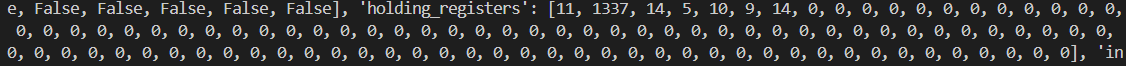
\includegraphics[width=1\textwidth]{images/AfterFabrication.png}
    \caption{Register after the fabrication attack}
    \label{fig:afterFabrication}
\end{figure}
\subsection{Modification attack}
The aim of this attack is to intercept the packet sent by the master to write in multiple registers 
and modify the value of one of them, and also delaying the response.
When a packet with the function code 16 is sent, the attacker will intercept it and modify 
the value of the register and send it to the server.
For this attack, after starting the slave, run the master with the function \texttt{master\_write()} and \texttt{master\_read()} 
to see the registers as in figure. Then run the \texttt{modification.py} script and with the master 
read the registers again to see the modification.
In the following image \ref{fig:beforeModification} we can see the register of 
interest before the attack:
\begin{figure}[h]
    \centering
    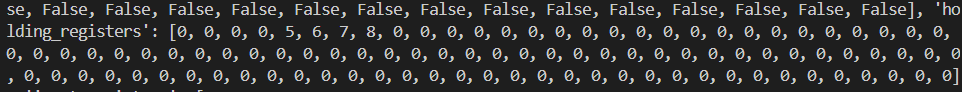
\includegraphics[width=1\textwidth]{images/BeforeModification.png}
    \caption{Register before the modification attack}
    \label{fig:beforeModification}
\end{figure} \\
After the modification, the value of the register is changed as shown in the 
following image \ref{fig:afterModification}:
\begin{figure}[h]
    \centering
    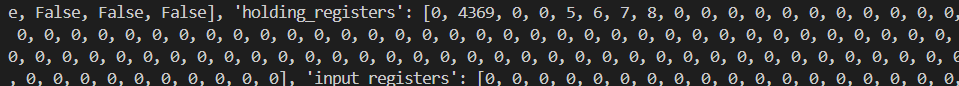
\includegraphics[width=1\textwidth]{images/AfterModification.png}
    \caption{Register after the modification attack}
    \label{fig:afterModification}
\end{figure} \\
In this case the original packet sent by the master is not blocked, but the aim is achieved anyway 
because the value of the register is changed starting from the packet sent by the master.
\begin{figure}[h]
    \centering
    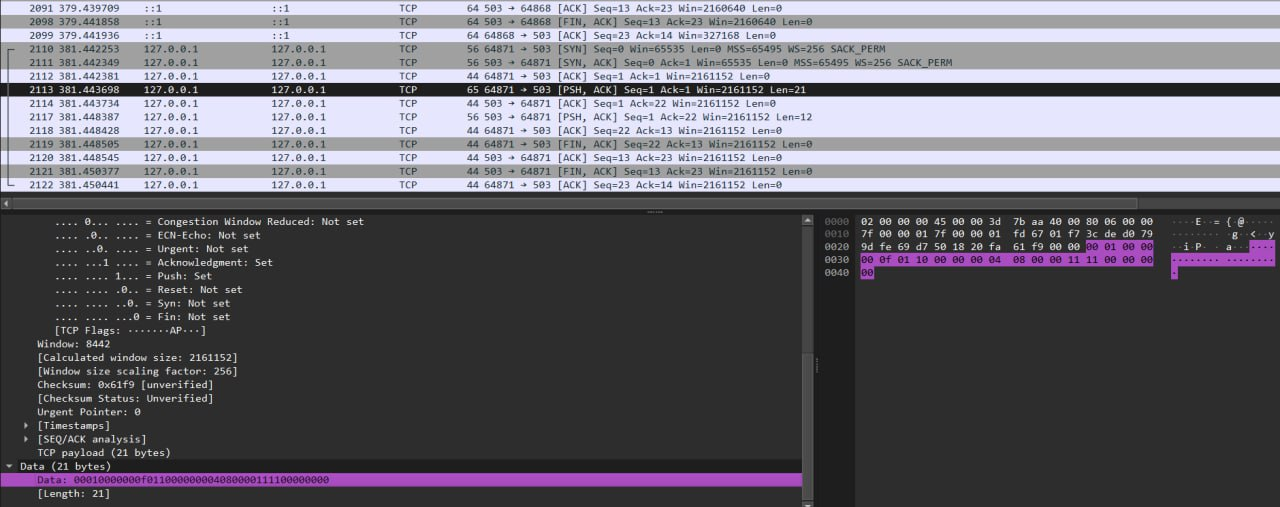
\includegraphics[width=1\textwidth]{images/wiresharkModification.jpg}
    \caption{Packet exchanged in the modification attack}
    \label{fig:wiresharkModification}
\end{figure} \\
As we can see in the image \ref{fig:wiresharkModification} the packet is sent 
to the server with two seconds of delay (id 2099-2110) 
and in the bottom-rigth section, higlighted in purple,
there are the values x11x11 that have been modified by the attacker.
\subsection{Interruption attack}
The aim of this attack is to interrupt the communication between the master and the slave by sending a 
flood of TCP FIN packets. The idea is to send so many packets that the server will be overloaded and
will not be able to respond to the master.
After starting the slave, run the \texttt{interruption.py} script and then the master 
with the function \texttt{master\_connected()}.
The idea was to create a TCP FIN packet (which is the flag that indicates the end of the connection)
and send it to the server with multiple threads in order to create also multiple requests 
at the same time.
This attack didn't work as expected, because the server was able to respond to the master anyway.
\begin{figure}[h]
    \centering
    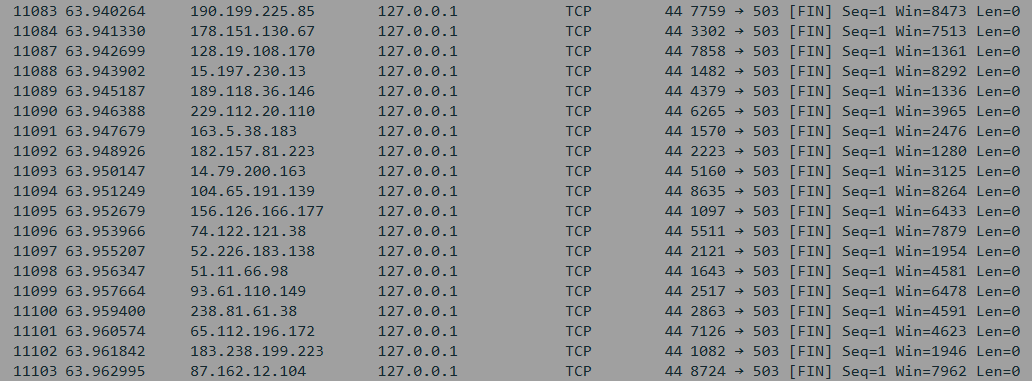
\includegraphics[width=1\textwidth]{images/wiresharkFINflood.png}
    \caption{Flood of TCP FIN packets}
    \label{fig:interruption}
\end{figure} \\
In the image \ref{fig:interruption} we can see a part of the flood of TCP FIN packets sent 
to the server, and effectively not all of them are responded by the server. However, if we run the master 
the server is still able to connect and respond to the request of the master.
We supposed that the server is able to manage the requests because of the implementation of the library 
\texttt{pymodbus}: we haven't found a way to determine if there is a maximum number of requests that 
the server can handle simultaneously, so it could work until the  resources are saturated.
\section{Conclusions}
In this work we have implemented four attacks on Modbus TCP networks, as described in the 
original paper \cite{huitsing2008attack}. Unfortunaltely, the interruption attack didn't work as expected.
We tried also other kinds of interruption attacks but we left in the final report only the most 
significant one. The other attacks worked as expected and we were able to intercept, 
modify and fabricate. This work allowed us understand how vulnerable the Modbus protocol is.
\printbibliography 


\end{document}
